\documentclass[11pt,a4paper]{article}
\usepackage[T1]{fontenc}
\usepackage{amsmath,amssymb,newtxtext,newtxmath}
\usepackage[margin=25mm]{geometry}
\usepackage{booktabs,tabularx,array,enumitem,microtype,caption}
\usepackage{tikz}
\usetikzlibrary{arrows.meta,positioning,calc}
\usepackage{xurl,hyperref}
\hypersetup{colorlinks=true,urlcolor=black,linkcolor=black,citecolor=black,
  pdftitle={Bailey(ing) Out}}
\captionsetup{font=small,labelfont=bf}
\setlength{\parindent}{1.2em}
\setlength{\parskip}{2pt}
\setlist{itemsep=2pt,topsep=4pt}
\newcommand{\clip}{\operatorname{clip}}
\newcommand{\ind}{\mathbf{1}}
\newcommand{\eps}{\varepsilon}
\title{Bailey(ing) Out}
\author{}
\date{}
\begin{document}
\maketitle
\vspace{-2em}

\begin{abstract}
The evacuation of Bailey Hall depends on the available exits, the flow permitted by aisles and doors, and the decisions occupants make as congestion develops. The model represents 1,329 people moving through a network of walkways with finite capacity and storage. Individual walking speeds, response times, familiarity, and companions affect movement, while Crowd Managers and signs provide guidance and removable barriers alter circulation. The formulation distinguishes physical delays from the delays people can observe and describes the assumptions used where Bailey-specific measurements are unavailable.
\end{abstract}

\section{Introduction}

Bailey Hall is a semicircular auditorium at Cornell University, with the orchestra and mezzanine on the first floor and the balcony above. The full audience consists of 1,329 people: 527 in the orchestra, 486 in the mezzanine, and 316 in the balcony, including three wheelchair users. Six access points connect the orchestra to the mezzanine. Nine doors lead from the auditorium to the curved outer corridor, which in turn connects to the foyer and side porticoes. The balcony is served by stairways near the foyer and emergency routes beside the stage. Most visitors ordinarily leave through the foyer and its exterior staircase, although the porticoes provide additional routes to street level. The elevator at the west side of the foyer is excluded from emergency evacuation. The geometry and these restrictions come from the Bailey Hall problem description and accompanying plans \cite{brief}.

The seating plan is approximately symmetric about the centre of the auditorium. Interior photographs show the wide common space, visible auditorium doors and exit signs, and clear views across much of the lower seating area. The raised mezzanine and the walls beyond its doors still separate the auditorium from the outer corridors. Occupants are therefore assumed to know the signed exit routes serving their level, without seeing the queues or obstructions beyond those doors. This distinction is consistent with Fu, Liu, and Liu's findings that visibility and familiarity influence attention to emergency exits and subsequent route choice \cite{brief,fu2023,fu2024}.

The reference case is a full concert. Under the staffing rule in the problem statement, at least one Crowd Manager is required for every 250 attendees, so a full audience of 1,329 requires at least six. Six is the baseline, not a maximum: additional managers can be considered at separate posts without changing the audience or physical capacities. During regular lectures, the problem assumes no Crowd Managers and greater student familiarity with the building \cite{brief}.

A short path is not necessarily a fast one. Many visitors may head toward the foyer because it is familiar, even if a side exit has a shorter queue. Others may hesitate at the alarm, wait for companions, or discover only partway through their route that a door is blocked. The model therefore combines movement through a network with individual exit decisions. Spearpoint and Xiang compared a network model with evacuations from university lecture theatres and found that accounting for restrictions at aisles and doors was important for reasonable clearance-time predictions \cite{spearpoint}. The representation retains aisle and door bottlenecks without simulating individual body contacts.

The principal outcome is the time between the evacuation announcement and the last occupant crossing the building's exterior boundary. Arrival at street level is recorded separately, particularly for people requiring assisted descent. The problem sets a benchmark of 180 seconds for building clearance \cite{brief}. It is not used to calibrate movement parameters.

\section{Key Assumptions}

The following assumptions define the scope of the model.
\begin{enumerate}[label=\arabic*.]
\item \textbf{Geometry.} Routes follow the seating rows, longitudinal aisles, transverse cross-aisles, corridors and stairs shown in the plans. The short stepped passage joining the outer transverse cross-aisle to the inner seating-block circulation is treated as a public connector, not a restricted seating row. It does not provide wheelchair access. People cannot cut through seats or walls \cite{brief}.

\item \textbf{Audience.} Walking speeds and response times vary among individuals. The reference audience includes $20\%$ adults aged at least 65. This approximates a mixed-age university concert, but is not a demographic estimate for Bailey Hall: the national share of older adults is about $18\%$, whereas particular music audiences may be much older \cite{census,nidi}. The audience mix is therefore varied separately rather than treated as known.

\item \textbf{Response.} Recognition and movement preparation are represented by separate delays. The main hall is treated as one alarmed space, without assigning separate alarm-arrival times to seating sections. There is no additional, explicitly sampled belongings-collection delay; brief individual actions are encompassed by the response-time distribution. Hopkin, Galea, and Deere observed substantially longer pre-movement times and frequent coat-related actions in a real theatre evacuation, so the reference represents prompt, clearly directed departure rather than their measured audience \cite{hopkin}.

\item \textbf{Movement.} Links have finite flow and storage. Congestion develops when a downstream link or doorway cannot admit people as quickly as they arrive. Spacing and time-headway observations motivate this network approximation; contacts, pushing, and falls are not resolved \cite{seyfried,johansson}.

\item \textbf{Information.} Occupants initially know the signed auditorium exits serving their level but not the conditions along the corresponding exterior routes. This relatively favourable starting knowledge reflects the open room and visible signs without implying a view through the surrounding walls. Familiarity and visual attention can still bias choices among known doors \cite{fu2023,fu2024}.

\item \textbf{Social behaviour.} Nearby people can accelerate initial recognition, while companions may wait for one another and coordinate their routes. General crowd imitation does not continue to alter route preferences after departure; later social coordination is restricted to identified companions. This distinction follows evidence that groups affect early response and approach more clearly than discharge through a door \cite{bode}.

\item \textbf{Interventions.} Managers and signs change information, not passage capacity. Only low or visually transparent barriers are considered, so installations do not obscure the stage, exit openings, or neighbouring circulation. They can still reduce usable width or lengthen a route \cite{feliciani,wang}.

\item \textbf{Accessibility.} Three wheelchair users remain in the population, and the elevator is excluded as instructed in the problem. Backstage and ground-level spaces are outside its scope. Assistance is represented separately from walking on stairs \cite{brief,mobility}.
\end{enumerate}

Numerical choices without venue measurements are stated where they enter the model. Published studies motivate the mechanisms but do not provide a fitted parameter set for Bailey Hall.

\section{Model Formulation}

\subsection{Navigation Network and Occupant State}

Let $V$ denote junctions at aisle intersections, doors, stair connections, and changes in direction, and let $E$ denote the walkway links. The navigation network is the directed graph
\begin{equation}\label{eq:graph}
G=(V,E).
\end{equation}

A link $e$ has walking length $L_e$, horizontal length $L_{e,\mathrm{plan}}$, usable width $w_e$, lane count $m_e$, floor, and permitted direction. Its path follows the reconstructed walkway. A person may leave a seating row through its ends but cannot use a different row as a shortcut. Closed and inaccessible links are excluded from the set of feasible routes \cite{spearpoint}.

The orchestra seating plan shows transverse cross-aisles dividing the outer seating blocks. At the middle break, the outer cross-aisle meets the curved longitudinal aisle and continues through a short stepped opening into the inner seating-block circulation. The stair-like treads and bounded opening in the enlarged plan, together with the open internal circulation visible in photographs, identify this as a passage rather than a row of seats. The same arrangement is represented on the opposite side where the plan shows its corresponding opening. In the network, this connection joins the neighbouring aisles, allowing movement between seating blocks without passing through occupied rows. Its stepped section uses stair travel and service rules and is unavailable to wheelchair users; the accessible route remains elsewhere in the network \cite{brief}. The dimensions are taken from the drawn clear passage, not from the adjacent seating-row measurements.

\begin{figure}[htbp]
\centering
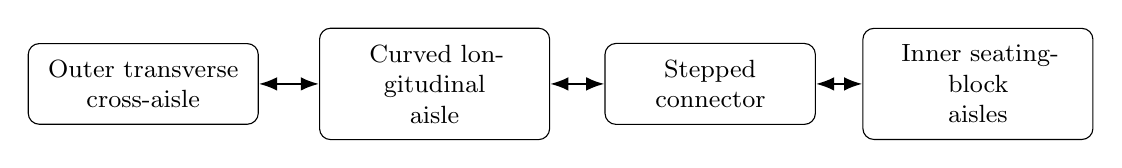
\begin{tikzpicture}[>=Latex, every node/.style={font=\small}]
\node[draw,rounded corners,inner sep=6pt,align=center,text width=2.5cm] (outer) at (0,0) {Outer transverse\\cross-aisle};
\node[draw,rounded corners,inner sep=6pt,align=center,text width=2.5cm] (curve) at (3.7,0) {Curved longitudinal\\aisle};
\node[draw,rounded corners,inner sep=6pt,align=center,text width=2.25cm] (steps) at (7.2,0) {Stepped\\connector};
\node[draw,rounded corners,inner sep=6pt,align=center,text width=2.5cm] (inner) at (10.6,0) {Inner seating-block\\aisles};
\draw[<->,thick] (outer)--(curve);
\draw[<->,thick] (curve)--(steps);
\draw[<->,thick] (steps)--(inner);
\end{tikzpicture}
\caption{Orchestra cross-aisle connection. It is part of the circulation network, with a stepped transition and no through-route across seating rows. Schematic, not to scale.}
\label{fig:crossaisle}
\end{figure}

The model distinguishes seven exterior exit groups: the foyer; the west and east porticoes; the west and east stage routes; and the northwest and northeast balcony exits. The seven groups follow the building plans \cite{brief} and retain distinct queues and familiarity levels.

Each occupant begins at a seat with a walking speed, response delay, social group, and exit preference. The principal states are recognition, response, waiting for companions or row access, movement, queuing, and departure. The separate belongings-preparation state is omitted; the model accounts for leaving a seat through travel along its row, but does not add time for collecting possessions. An assisted occupant may reach the exterior before reaching street level.

\begin{figure}[htbp]
\centering
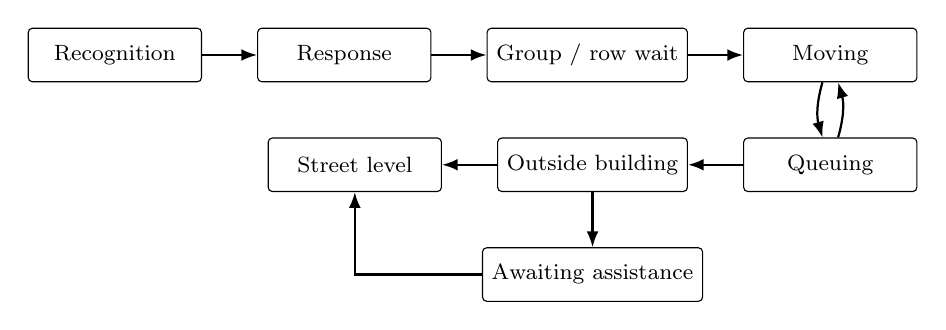
\begin{tikzpicture}[node distance=7mm and 7mm,
 state/.style={draw,rounded corners=1.5pt,align=center,font=\footnotesize,minimum width=2.2cm,minimum height=.68cm},
 arr/.style={-{Latex[length=2mm]},thick}]
\node[state] (r) {Recognition};
\node[state,right=of r] (p) {Response};
\node[state,right=of p] (w) {Group / row wait};
\node[state,right=of w] (m) {Moving};
\node[state,below=of m] (q) {Queuing};
\node[state,left=of q] (o) {Outside building};
\node[state,left=of o] (s) {Street level};
\node[state,below=of o] (a) {Awaiting assistance};
\draw[arr] (r)--(p);\draw[arr] (p)--(w);\draw[arr] (w)--(m);
\draw[arr] (m) to[bend right=16] (q);\draw[arr] (q) to[bend right=16] (m);
\draw[arr] (q)--(o);\draw[arr] (o)--(s);\draw[arr] (o)--(a);\draw[arr] (a)-|(s);
\end{tikzpicture}
\caption{Occupant states. Building departure and arrival at street level are recorded separately.}
\label{fig:states}
\end{figure}

\subsection{Audience Characteristics}

Each ambulatory occupant $i$ receives a free walking speed $v_{0i}$. Let $Z_i$ be a standard normal draw, $\mu=1.40$ m/s the reference mean for non-older adults, $\sigma=0.18$ m/s its standard deviation, and $f_i=0.85$ for occupants aged at least 65 and $1$ otherwise. The operator $\clip_{[a,b]}(x)$ restricts a value to $[a,b]$. Then
\begin{equation}\label{eq:speed}
v_{0i}=\clip_{[0.5,2.0]}\!\left[f_i(\mu+\sigma Z_i)\right],
\qquad Z_i\sim\mathcal N(0,1).
\end{equation}
The reference older share is $20\%$, and the three wheelchair users have a separate free speed of $0.8$ m/s. Murtagh and colleagues report mean outdoor speeds of $1.31$ m/s at a usual pace and $1.47$ m/s at a medium pace, placing the $1.40$ m/s assumption between them \cite{murtagh}. Indoor walking experiments by Daamen and Hoogendoorn report observed and estimated free-speed spreads ranging from roughly $0.15$ to $0.25$ m/s in several flow arrangements, making $0.18$ m/s a reasonable single-group spread \cite{daamen}. In the Rotterdam Study, the mean gait speed of community-dwelling older adults was $1.20$ m/s; the factor $0.85$ gives approximately $1.19$ m/s before clipping \cite{dommers,bohannon}. These are walking speeds before congestion, not speeds in a crowded aisle or on stairs. The age mix and the transfer from these studies to a concert remain assumptions.

For ambulatory occupants, effective body radius is normally distributed with mean $0.22$ m and standard deviation $0.02$ m, bounded by $0.17$ and $0.30$ m. The wheelchair radius is $0.45$ m. These are approximate space requirements. Speed on stairs is multiplied by $0.57$ for ordinary walkers and $0.51$ for older walkers, with any scenario-specific environmental factor. NIST measurements show that stair movement differs substantially from free corridor walking, although they do not establish these multipliers for Bailey Hall \cite{nist}.

\subsection{Recognition, Response, and Group Behaviour}

Recognizing an alarm and deciding to move are treated as separate delays. Hopkin, Galea, and Deere found that response times in a theatre were strongly right-skewed and depended in part on seat location \cite{hopkin}. A delay $\tau$ with median $m$ and logarithmic standard deviation $s$ is represented as
\begin{equation}\label{eq:lognormal-time}
\tau=\exp(\log m+sZ),\qquad Z\sim\mathcal N(0,1).
\end{equation}
Recognition has median $6$ s and logarithmic standard deviation $0.6$. The subsequent response delay has median $14$ s and the same logarithmic standard deviation. No additional linear correction for distance from the aisle or a balcony seat is imposed: both factors already affect travel through the reconstructed network. Hopkin, Galea, and Deere found that pre-movement behaviour varies among occupants and may depend on seat location, but their study does not establish a distance coefficient transferable to Bailey Hall \cite{hopkin}. The chosen $6$ s and $14$ s medians describe a clearly signalled, prompt-response case. They are appreciably shorter than the mean time to movement observed in the unannounced Marlowe Theatre evacuation, where Galea and colleagues reported $55.6$ s for non-disabled participants excluding helpers \cite{galea2017theatre}. The study measured the full interval preceding movement rather than these two clocks separately. Faster recognition ($3$ s) and response ($8$ s), together with a slower pre-movement scenario, remain comparison cases rather than calibrated alternatives.

There is no separate random draw for retrieving coats or personal belongings. The general response delay covers ordinary hesitation and brief preparation, but not prolonged retrieval. In the Marlowe Theatre study, $39\%$ of the observed population collected or put on coats, so omitting an explicit retrieval phase may shorten predicted times \cite{galea2017theatre}. It cannot be defended by analogy with an aircraft; the reference instead represents a scenario with clear instructions to depart without collecting possessions.

Initial recognition may accelerate as nearby occupants begin reacting. Let $\phi_i\in[0,1]$ be the fraction of occupant $i$'s original seat neighbours who have begun responding or moving, and let $c_i(t)$ denote progress through the recognition phase. During that phase,
\begin{equation}\label{eq:social}
\frac{dc_i}{dt}=1+\phi_i.
\end{equation}
Only the initial recognition clock is affected; later route decisions do not depend on the movement of unrelated distant occupants. The local influence is consistent with observed social cues during evacuation, while the unit coefficient is a modest modelling assumption rather than a measured response factor \cite{bode,fu2023}.

About half the audience belongs to groups of two to four. Of these groups, $70\%$ are pairs, $20\%$ consist of three people and $10\%$ of four. Members sit near one another, may wait for companions for at most $20$ s, and normally adopt the leader's destination unless an accepted safety instruction or an inaccessible route requires a change. Pairs are more common than larger groups because coordination between one or two companions is a plausible concert-going pattern; the shares are not measured for Bailey Hall. The waiting cap is shorter than a prolonged search because the group begins in adjacent seats and encounters the same alarm. Bode and colleagues found that groups mainly influence response and approach rather than the capacity of the final exit \cite{bode}. Group members already on the same link may also pace one another locally, as described below.

\subsection{Walking Service and Finite Storage}\label{sec:transport}

Each link $e$ has walking-service capacity $C_e^{\mathrm{walk}}$ (persons/s) and storage limit $S_e$ (persons). Here $m_e$ is its lane count, $\bar v_e$ its representative speed, $d_b=0.44$ m the assumed mean body diameter, $H=0.7$ s the following headway, and $\rho_{\max}=4.5$ persons/m$^2$ the storage density. Define $\gamma_e=L_{e,\mathrm{plan}}/L_e$, which converts walking length to horizontal length. Then
\begin{equation}\label{eq:link}
C_e^{\mathrm{walk}}=\frac{m_e\bar v_e}{d_b+H\bar v_e},\qquad
S_e=\max\!\left(m_e,\left\lfloor \rho_{\max}L_ew_e\gamma_e\right\rfloor\right),
\qquad\rho_{\max}=4.5\ \mathrm{persons/m^2}.
\end{equation}
For stairs, $\mathrm{drop}_e$ is the vertical drop and $L_e=\sqrt{L_{e,\mathrm{plan}}^2+\mathrm{drop}_e^2}$. The lower bound $S_e\ge m_e$ allows one person per lane on short links, even where this exceeds the area-based density. Storage does not represent contact pressure.

The flow formula comes from an assumed spacing of $d_b+H\bar v_e$ between successive pedestrians: dividing speed by that spacing gives a per-lane passage rate. Seyfried and colleagues studied how pedestrian spacing and density relate to speed, while Johansson identified approximately constant net-time headway as an important feature across several datasets \cite{seyfried,johansson}. The $0.7$ s headway gives a finite separation between successive pedestrians even when they walk quickly, while $4.5$ persons/m$^2$ is an upper storage assumption used to prevent unbounded accumulation on short passage links. Neither quantity is measured for Bailey Hall, and storage density should not be interpreted as a safe operating density.

Where the plan does not specify lanes, the reconstructed width determines an approximate count:
\begin{equation}\label{eq:lanes}
m_e=\max\!\left(1,\left\lfloor \frac{w_e}{0.6\ \mathrm{m}}\right\rfloor\right)
\qquad\text{for a traversable link}.
\end{equation}
The nominal $0.6$ m lane width is a geometric convention, not a measured queue spacing. Each person must still fit through the actual link; in particular, wheelchair accessibility cannot be inferred from $m_e$ alone. Seat rows have their own body-spacing storage and release people through their two ends. They cannot be used to pass between aisles. No additional fixed speed cap is assigned to an occupied row. Spearpoint and Xiang found that a separate row-speed reduction generally overpredicted lecture-theatre clearance times when aisle and doorway restrictions were already represented \cite{spearpoint}. The representative speed in Eq.~\eqref{eq:link} uses the configured free-speed mean and the applicable corridor or stair factor; faster walkers can therefore affect both link travel time and potential service.

The two directions of a passage cannot independently claim its full capacity. Let $m_{e,+}$ and $m_{e,-}$ be the numbers of logical lanes assigned to outgoing and opposing streams. When only one direction is active, it may use all $m_e$ lanes. If both are active on a link with at least two lanes, lanes are divided as evenly as possible, with any extra lane assigned to the direction whose queue has been waiting longer. An occupied lane is not reassigned before its users have cleared it. With $\delta\in\{+,-\}$ denoting direction, the available service is
\begin{equation}\label{eq:direction}
C_{e,\delta}^{\mathrm{walk}}=
\frac{m_{e,\delta}\bar v_e}{d_b+H\bar v_e},
\qquad m_{e,+}+m_{e,-}\leq m_e.
\end{equation}
On a one-lane passage, entry is restricted to one direction at a time until it clears. This is an integer-lane approximation of self-organized counterflow, rather than a calculation of individual avoidance. Feliciani, Murakami, and Nishinari showed that bidirectional capacity depends on both opposing-flow conflicts and lane formation \cite{feliciani2018}. Their results support accounting for shared capacity, not the precise lane-assignment rule used here. In all cases, the combined directional service cannot exceed the physical passage capacity.

Doors and stair entrances have an additional admission limit. Let $q_e$ be their specific flow in persons/(m s), $b_e$ the boundary width lost at each side of an opening, and $f_{\mathrm{env}}$ an environmental factor (one in the reference scenario). Define $[x]_+=\max(0,x)$. The effective width and maximum gate service are
\begin{equation}\label{eq:gate}
w_{e,\mathrm{eff}}=[w_e-2b_e]_+,
\qquad C_e^{\mathrm{gate}}=q_ew_{e,\mathrm{eff}}f_{\mathrm{env}}.
\end{equation}
The baseline takes $q_e=1.3$ persons/(m s) and $b_e=0.15$ m for doors, and $q_e=1.0$ persons/(m s) and $b_e=0.09$ m for stair passages. For stair flights divided into $m_e$ lanes, the aggregate usable width is $m_e[w_e/m_e-2b_e]_+$. These specific flows lie within commonly used engineering ranges: Gwynne and colleagues report the SFPE doorway value of $1.3$ persons/(m s) and stair rates of approximately $0.94$--$1.16$ persons/(m s) \cite{gwynne}. The effective-width correction is a standard simplifying convention, but actual door operation and leaf geometry can alter throughput \cite{gwynne}. In particular, if the effective width is zero, the gate has no service; an arbitrary minimum positive width is not introduced. No separate urgency or luggage multiplier is applied.

Flow through a passage is limited by both its walking-service rate and any gate at the next link. People are admitted in their arrival order, with fractional service carried between short time intervals so that the nominal capacity is not rounded to zero at each interval. Actual congestion is determined by these rates and by downstream storage, not by an additional perceived-density penalty.

Let $n_e^k$ be the number on link $e$ at step $k$ and $A_e^k,D_e^k$ the admissions and departures during that step. Occupancy satisfies
\begin{equation}\label{eq:occupancy}
n_e^{k+1}=n_e^k+A_e^k-D_e^k,\qquad 0\leq n_e^k\leq S_e.
\end{equation}
A person occupies storage even while travelling along the link. A full downstream link blocks transfers and causes queue spillback. At a junction, entry in either direction is permitted only when the assigned lane and the receiving link have enough space; counterflow never creates additional storage or service.

Within each lane, waiting people are served in their order of arrival; the ends of a seating row are ordered by their individual readiness times. Someone who has not completed the link's walking time cannot yet enter its discharge queue. Different lanes may advance independently, but a formed doorway queue cannot be overtaken. The model thus separates travel along a passage from waiting to leave it.

Companions who remain on the same link, travel in the same direction, and are within $4$ m of one another adopt the slowest member's free speed. Farther-separated members do not hold an entire group to that pace. Bode and colleagues' observations suggest that much of the effect of social groups occurs before the final bottleneck, which supports representing this coordination locally \cite{bode}; the $4$ m threshold is an assumed range. Let $\ell_i^k$ denote a walker's remaining distance on the current link, $v_i^k$ the current speed, and $t_i^{\mathrm{ready}}$ the projected completion time. Then
\begin{equation}\label{eq:remaining}
\ell_i^{k+1}=\max(0,\ell_i^k-v_i^k\Delta t),\qquad
t_i^{\mathrm{ready}}=t_k+\ell_i^k/v_i^k\quad(v_i^k>0).
\end{equation}
A person who has reached the end of a link still waits when downstream storage or service is unavailable. 

\subsection{Perception and Exit Choice}

The approximately symmetric auditorium and the visible exit signs make the auditorium doors relatively easy to locate. The interior photographs show long sightlines across the lower seating, but the raised mezzanine and perimeter walls conceal much of the circulation beyond those doors. The reference case therefore assumes knowledge of the signed exits serving each person's level, not sight of every exterior doorway, queue, or obstruction. Fu, Liu, and Liu found that familiarity and visual attention affect use of available exits \cite{fu2023,fu2024}. Thus knowing an exit exists does not determine whether it is selected, and sign detection is not used to teach an exit that the occupant already knows.

At each junction, person $i$ estimates the walking time to a candidate exit group $g$ along connected, accessible links. Let $\mathcal P_{ig}$ be the set of feasible paths to $g$, $v_{ie}$ the expected free speed of person $i$ on link $e$, and $\mathcal V_i(t)$ the gates whose queues are directly visible to that person at time $t$. A gate is visible only on the same floor, within $15$ m, and without a wall or column across the sightline. Let $\widehat Q_{ie}(t)$ count visible waiting occupants and let $C_e^{\mathrm{gate}}$ be the nominal gate capacity. The perceived route time is
\begin{equation}\label{eq:perceived}
\widehat T_{ig}(t)=\min_{P\in\mathcal P_{ig}}
\left\{\sum_{e\in P}\frac{L_e}{v_{ie}}+
\sum_{e\in P\cap\mathcal V_i(t)}\frac{\widehat Q_{ie}(t)}{C_e^{\mathrm{gate}}}\right\}.
\end{equation}
The first term depends on the occupant's position and physical route lengths. The second adds delay only at a gate whose queue can be seen. There is no separate penalty based on the total number of people somewhere along an ordinary aisle. They still cause physical queues through the service and storage constraints in Section~\ref{sec:transport}. Treating an unseen queue as unknown, rather than supplying its true length, avoids giving people perfect knowledge of the building. The $15$ m sight range is an assumed local observation distance; it does not assert that an actual line of sight is clear through a crowd.

Two broad preferences replace the six finely weighted behavioural categories. A proportion $p_T=0.65$ uses estimated route time as its main criterion, while $p_H=0.35$ has a preference for the familiar foyer. Let $H_i$ be $0$ seconds for a time-oriented occupant and $12$ seconds for a familiarity-oriented occupant. Let $F_g=1$ for the foyer and $0$ for other exits. Finally, $\varepsilon_{ig}$ is a fixed Gumbel preference draw, with scale $4$ seconds, for each occupant--exit pair. The perceived utility is
\begin{equation}\label{eq:utility}
U_{ig}(t)=-\widehat T_{ig}(t)-H_i(1-F_g)+\varepsilon_{ig},
\qquad g_i=\arg\max_{g}U_{ig}(t).
\end{equation}
Fixed random utility allows two people with similar routes to make different choices without independently redrawing their tastes at every junction \cite{train}. Experiments support the existence of travel-time and familiarity preferences, not a particular population split \cite{liao,fu2024}. The $65/35$ split, $12$ s familiarity allowance, and $4$ s preference dispersion are therefore illustrative, not values estimated by the cited experiments. A balanced preference split is a useful alternative because no observed Bailey Hall choice frequencies are available. People travelling with companions normally retain the leader's destination, so companionship is represented separately rather than through another arbitrary behavioural type. Accepted guidance takes priority over either preference when it identifies a feasible exit.

Choices may be reconsidered upon reaching a junction, encountering a visible queue, receiving new guidance, or learning that a planned link is closed. To avoid reacting to very small estimates, a person switches from the current destination $g$ to a new destination $h$ only if
\begin{equation}\label{eq:review}
U_{ih}(t)-U_{ig}(t)\geq8\ \mathrm{s}.
\end{equation}
The eight-second margin represents inertia in the presence of uncertain queue estimates, not a measured switching threshold. In Liao and colleagues' experiments, people who changed exits formed only about $0$--$7.5\%$ of participants within individual runs, despite opportunities for reconsideration \cite{liao}. Reviews therefore occur at junctions or after meaningful new information, but they do not force frequent switching. A smaller $5$ s margin represents a more adaptive alternative, rather than an established typical response. Any chosen destination becomes effective only at a connected junction; it cannot reverse completed travel or take a shortcut through seating.

\subsection{Managers and Announcements}

The baseline concert includes six Crowd Managers, the minimum specified for 1,329 attendees \cite{brief}. Additional managers can occupy distinct posts. Each becomes active after a lognormal delay with median $10$ s and logarithmic standard deviation $0.5$. A spoken instruction can reach an occupant on the same floor within $12$ m, provided no represented wall blocks the acoustic path. Let $h=0.35$ s$^{-1}$ be the hearing rate, $u_i^{CM}$ a fixed uniform draw for occupant $i$, and $A_i^{CM}$ its acceptance indicator. The probability of hearing during an exposure interval $\Delta t$ and the chance of accepting a heard instruction are
\begin{equation}\label{eq:manager}
p_{\mathrm{hear}}(\Delta t)=1-e^{-h\Delta t},\qquad
A_i^{CM}=\ind\{u_i^{CM}<0.85\},\qquad u_i^{CM}\sim U(0,1).
\end{equation}
Hearing and acceptance remain distinct. The $12$ m range confines each manager's influence to a local part of the open hall, and the persistent draw avoids making compliance inevitable after repeated instructions. The $85\%$ acceptance assumption represents a relatively high but incomplete response to a clear instruction from trained staff. In an analysis of 126 real-emergency videos, van der Wal and colleagues found that staff guidance was associated with less delayed response than alarms alone; their analysis did not measure the probability that a given person complied \cite{vanderwal}. Mayr and K\"oster studied routing with limited compliance, supporting its treatment as an uncertain behavioural parameter rather than perfect obedience \cite{mayr}. Neither study establishes $85\%$ for Bailey Hall; a $70$--$90\%$ range represents different levels of trust and instruction clarity.

Hearing an instruction brings an occupant who has not yet recognized the alarm into the response phase. Accepting a feasible destination recommendation takes precedence over an ordinary route preference, but cannot overcome a blocked corridor or inaccessible stair. Subsequent consistent instructions reinforce the destination; a newly discovered obstruction may require another choice. A manager is modelled as a source of information, not as an extra body occupying doorway capacity.

An optional pre-announcement reaches $60\%$ of the audience, and $70\%$ of those reached accept its suggested seat-block exit. Reach means successful reception and attention, not that the public-address system is inaudible to others. A recommendation does not cancel the ordinary recognition, response, or companion-waiting delays. These rates are assumptions for an advance-information scenario, not measured effects.

Managers can remain at their posts or walk between connected, level, non-gated corridor locations at an assumed $1$ m/s, provided the route is at least $1.8$ m wide and not occupied in a way that prevents passage. Liu and colleagues distinguish stationary and moving guide effectiveness and show that placement matters \cite{liu}. The chosen patrol speed and width screen keep the range of staff instructions physically limited without resolving detailed staff--audience contacts.

\subsection{Exit Signs and Dynamic Guidance}

Directional signs make the known exits easier to locate and can recommend a different route. A wall sign occupies a point and has a facing direction; an LED strip follows a polyline along an existing walkway. Each installation has a location, activation time, viewing range, detection probability, acceptance probability, and public exit message. Static installations retain their message, while dynamic signs may update it. The distinction between making a sign visible and making its guidance persuasive follows the signage experiments of Galea and colleagues \cite{galea2014}. Legibility is represented through visibility and detection rather than a detailed model of illumination or eye movement.

A wall sign is visible only when it is active, on the observer's floor, within range, in front of the sign, and not hidden by a represented wall or column. Let $\mathbf y_j$ and $\mathbf f_j$ be sign $j$'s position and facing unit vector, $\mathbf x_i$ the occupant's position, $R_j$ its viewing radius, and $\alpha_j$ its facing half-angle. Let $I_{\mathrm{floor}}$, $I_{\mathrm{range}}$, $I_{\mathrm{facing}}$, $I_{\mathrm{clear}}$, and $I_{\mathrm{active}}$ be indicators of, respectively, floor agreement, distance, facing, an unobstructed sightline, and activation. Their product $E_{ij}$ indicates geometric eligibility to see a sign:
\begin{align}\label{eq:visibility}
E_{ij}&=I_{\mathrm{floor}}I_{\mathrm{range}}I_{\mathrm{facing}}I_{\mathrm{clear}}I_{\mathrm{active}},\\
I_{\mathrm{range}}&=\ind\{\|\mathbf x_i-\mathbf y_j\|\leq R_j\},\\
I_{\mathrm{facing}}&=\ind\!\left\{\mathbf f_j\cdot
\frac{\mathbf x_i-\mathbf y_j}{\|\mathbf x_i-\mathbf y_j\|}\geq\cos\alpha_j\right\}.
\end{align}
If the observer occupies the sign's point, the facing condition is satisfied. For a strip, visibility is checked along its segments at points no more than $0.5$ m apart, without a facing cone. Walls and columns can block sight, but head occlusion and gaze direction are not modelled.

Added LEDs activate after $3$ s, are visible within $8$ m, and, for wall signs, have a $70^\circ$ half-angle. Their detection probability is $0.77$ and their acceptance probability is $0.8$. Existing exit signs are assigned detection probability $0.38$. Galea, Xie, and Lawrence observed conventional signs being noticed by $38\%$ of participants and tested dynamic signs by $77\%$ in a controlled unfamiliar-building setting \cite{galea2014}. These are transferred detection values, not Bailey Hall measurements. In that study, people who noticed the dynamic sign followed it; the present $0.8$ acceptance probability is a more cautious transfer to a crowded concert. The $3$ s activation represents rapid illumination after an alarm; the $8$ m range and $70^\circ$ cone limit influence to people with a plausible view of a sign. The $0.8$ acceptance value allows a noticed sign to be disregarded. The remaining placement and acceptance values are assumptions. No numerical smoke or darkness multiplier is imposed without optical measurements; reduced-visibility scenarios instead use separately stated detection assumptions. Galea and colleagues' later full-scale trials also suggest that voice messages and changing signs must be mutually consistent; they do not provide a second independent detection probability \cite{galea2017}.

For a particular person and sign, noticing and accepting are separate, persistent tendencies. Seeing the same unchanged message again does not automatically create another independent chance to notice it. A new message can be considered, but the underlying individual tendencies remain the same. Noticing a message gives information about the recommended direction; accepting it can commit the person to that exit if the route is accessible. If the message conflicts with an already accepted Crowd Manager instruction, the manager's instruction takes priority. This rule avoids simultaneously committing the same person to incompatible destinations.

Dynamic signs may change their messages when managers observe congestion or a blocked exit. An observation becomes available locally after $2$ s and reaches the sign controller after an additional $3$ s. The controller uses the most recent reports from managers with a view of the relevant gate; it does not see the true state of every corridor. Signs compare estimated route times with reported queues and change direction only if the alternative is at least $8$ s better and the current message has been displayed for $20$ s. This uses the same improvement margin as individual route reconsideration, while the holding time prevents rapid public-message reversals. The observation and reporting delays are modest scenario assumptions, not measured Bailey communication times. L\'opez-Carmona and Paricio Garc\'ia's adaptive guidance research supports responding to changing congestion rather than relying on a fixed assignment \cite{cellevac}. An LED strip points along the currently recommended route; its arrow changes when that route changes.

A manager who can see a gate is assumed to know its current queue and nominal service rate. Reports from other managers remain in use until replaced. If no report exists, the controller falls back to nominal route time rather than assuming that a gate is known to be empty. The model gives staff precise counts at gates they can see, but no instantaneous information about the whole building. Unexpected obstructions are learned only through local observation or a report.

\begin{figure}[htbp]
\centering
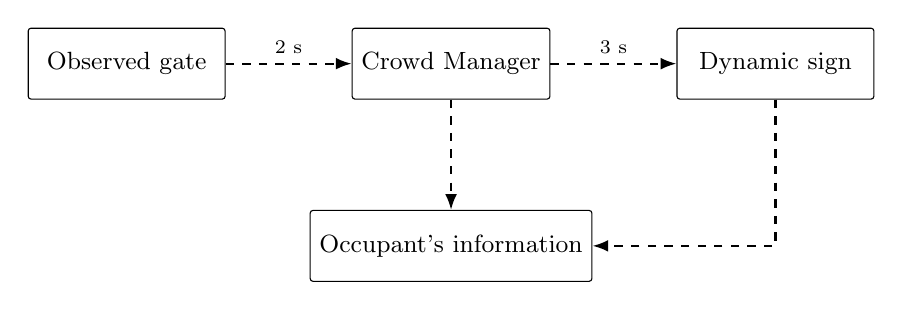
\begin{tikzpicture}[node distance=16mm,
  cell/.style={draw,rounded corners=1pt,align=center,minimum height=.9cm,
    minimum width=2.5cm,font=\small},
  arr/.style={-{Latex[length=2mm]},thick}]
\node[cell] (gate) {Observed gate};
\node[cell,right=of gate] (manager) {Crowd Manager};
\node[cell,right=of manager] (sign) {Dynamic sign};
\draw[arr,dashed] (gate)--node[above,font=\scriptsize]{2 s}(manager);
\draw[arr,dashed] (manager)--node[above,font=\scriptsize]{3 s}(sign);
\node[cell,below=14mm of manager] (viewer) {Occupant's information};
\draw[arr,dashed] (manager.south) -- (viewer.north);
\draw[arr,dashed] (sign.south) |- (viewer.east);
\end{tikzpicture}
\caption{Local gate observations reach the sign controller after a delay. Occupants receive guidance by hearing a manager or noticing a sign.}
\label{fig:information}
\end{figure}

\subsection{Temporary Barriers}

Temporary barriers are limited to low belts, ropes, and open railings that preserve sightlines toward the stage and nearby exits. Opaque panels are excluded. The model treats a barrier as a physical object that can redirect occupants, change walking distance, or reduce usable width, but never increase a doorway's service rate by itself.

For a barrier of length $b$ placed at angle $\theta$ to the corridor direction, let $w_e$ be the original corridor width. The projected obstruction and remaining bypass width are
\begin{equation}\label{eq:barrier}
w_{\mathrm{span}}=|b\sin\theta|,\qquad
w_{\mathrm{bypass}}=w_e-w_{\mathrm{span}}.
\end{equation}
The barrier is anchored along one side, leaving a single detour around its free end. The bypass follows the altered walkway rather than crossing the device. A positive bypass uses the same lane-width convention as Eq.~\eqref{eq:lanes} and the same walking-service rule as any other passage; an oblique barrier may also increase walking distance.
A barrier spanning the entire width closes the link. Devices are confined to identified corridor positions, away from seating rows and door thresholds. A partial bypass must remain at least $1.1$ m wide, and all wheelchair origins must retain an accessible path. This width is a modelling screen, not a statement of building-code compliance. Experiments by Wang and colleagues and by Feliciani and colleagues show that obstacle placement can improve or worsen flow depending on geometry and crowd conditions \cite{wang,feliciani,chen}. Consequently, no general percentage improvement is assigned to barriers.

\subsection{Assisted Evacuation}

The three wheelchair users retain access only to feasible routes. The west-foyer elevator is excluded from emergency evacuation under the problem statement \cite{brief}. Two assistance teams are assumed to become available after $60$ s, and assisted descent takes a lognormal time with median $60$ s and log standard deviation $0.4$. Research on stair evacuation by people with mobility impairments documents substantial differences among unaided, accompanied, and equipment-assisted movement \cite{mobility}. This supports representing assistance separately rather than assigning everyone an ordinary stair speed. Two teams represent scarce assistance rather than simultaneous help for every person; availability after $60$ s allows time for teams to reach their positions. A median descent of $60$ s with a lognormal spread allows assisted movement to be substantially slower and more variable than ordinary walking. These are scenario assumptions, not measurements of Bailey Hall staffing or assisted-descent times. An occupant can leave the building onto an exterior assistance landing before reaching street level, so those two times are recorded separately.

\subsection{Time Evolution of the Evacuation}

The evacuation evolves through discrete intervals of duration $\Delta t$. The reference interval is $0.1$ s, with a finer variant of $0.0125$ s. The finer interval tests how much discretization of queues and arrival times affects predictions without altering the physical model. Neighbour activity is considered during initial recognition; manager hearing is evaluated over simulated one-second intervals, while route reviews occur at meaningful decision points. These time scales describe the same continuous event at different levels of detail: walking and queue service need short steps, while recognition and communication change less frequently. The step sizes are numerical choices, not observed human reaction times.

Within an interval, visible queues and messages may change a person's intended destination. Recognition, response, and group waiting then progress; those already moving advance along the current walkway. Completing a link does not guarantee entry to the next one: the connection must be open and accessible, and both its storage and any relevant passage or gate service must be available. Otherwise the occupant remains upstream, allowing queues to extend backward through the building. This sequence couples individual decisions to the restrictions created by other people's movements.

If a person's speed changes while already on a link, the remaining distance is preserved and the completion time is recalculated using the new positive speed. A speed change neither resets the distance travelled nor allows someone to cross several positive-length links instantaneously.

For comparisons between interventions, a sampled audience retains the same seats, body sizes, speeds, response delays, groups, and persistent preferences. Only the arrangement of staff, signs, barriers, or instructions is changed. Common audience draws reduce sampling noise in paired comparisons, but not parameter uncertainty.

\section{Evaluation Metrics}

\subsection{Full-House Clearance}

The principal performance measure is the time when the last audience member crosses the building's exterior boundary. It is not the mean time taken by an individual: most people may be outside while a small group remains trapped by a queue or awaiting assistance. Let $t_{ir}$ denote occupant $i$'s first exterior crossing in audience replication $r$. For $N=1329$ occupants and $R$ replications,
\begin{equation}\label{eq:clearance}
T_r=\max_{1\leq i\leq N}t_{ir},\qquad
\overline T=\frac{1}{R}\sum_{r=1}^{R}T_r,\qquad
\widehat p_{180}=\frac{1}{R}\sum_{r=1}^{R}\ind\{T_r\leq180\}.
\end{equation}
The 180-second threshold is specified by the contest problem \cite{brief}; it is not used to calibrate the movement rules. If a replication still has people inside at the 900-second observation horizon, its clearance time is known only to exceed 900 seconds. It does not meet the target, and a mean computed only over completed replications must be described as conditional rather than as an unconditional average.

\subsection{Exit Use, Queues, and Density}

Two arrangements may have similar clearance times while producing different crowding patterns. The model therefore also records which exits are used, how long people wait, whether assistance is complete, and where queues accumulate. Because occupancy is represented on links, density is a link-average quantity:
\begin{equation}\label{eq:density}
\rho_e(t)=\frac{n_e(t)}{L_ew_e\gamma_e}.
\end{equation}
The recorded outputs include peak and time-varying link density, queue lengths and waiting times, exit usage, and completion of assisted descent. Time spent above a reference density of $2$ persons/m$^2$ may also be compared between layouts, but that value is an analytical reporting threshold rather than an injury threshold. The network cannot estimate contact forces or injury risk.

\section{Interpretation of Parameter Uncertainty}

The reference values describe a prompt, well-signalled concert departure, not a calibration to measured Bailey Hall evacuation times. The free-speed mean of $1.40$ m/s lies between usual and medium walking paces; $1.30$ m/s is a slower alternative \cite{murtagh}. The assumed $20\%$ older share is compared with differently composed audiences, including $10\%$, $35\%$, and $50\%$ older attendees, since the programme and attendance records are unspecified. The response medians of $6$ and $14$ s are shorter than the pre-movement delays observed in the Marlowe Theatre and require a slower-response comparison \cite{galea2017theatre}. Staff acceptance of $0.85$ is similarly compared with $0.70$ and $0.90$; these are assumed probabilities, not findings from staff-guidance experiments. Initial knowledge of signed exits, the two route-preference shares, the counterflow lane rule, sign-reporting delays, and the switching margin also remain assumptions. Such comparisons vary the model's inputs; they are not statistical confidence intervals derived from the literature.

\section{Limitations}

The geometry is reconstructed from architectural and seating plans, not from surveyed walkway measurements. The stepped cross-aisle is included as circulation between the outer and inner seating-block aisles; its width and change in elevation are approximated from the plans. It is not treated as a level accessible crossing or as a shortcut across seating rows. The photographs help distinguish open seating circulation from barriers, but cannot provide precise passage dimensions or verify exit hardware. The model consequently retains geometric uncertainty even though the cross-aisle's role as a pedestrian connection is fixed.

The audience is assumed to respond promptly and to walk briskly when unobstructed. Its age composition, route preferences, manager compliance and companion waiting have not been observed at Bailey Hall. Published work supports heterogeneous behaviour without fixing these numerical values. Other audience compositions, slower response, weaker guidance and less complete exit knowledge can change clearance times without changing the building.

Network congestion accounts for gate throughput, finite storage, and queue spillback, but not collisions, pushing, falls, injuries, or detailed interactions among seated neighbours. Low barriers preserve architectural sightlines but may still create local crowding. Sightline checks do not include heads blocking a view, detailed smoke optics, or the movement of staff through a tightly packed crowd. Assisted descent is estimated rather than measured in this building, and the omitted backstage and ground-level occupants remain outside the defined population.

The predicted clearance time is an estimate for the stated audience and scenario, not a certification of compliance with building or fire-safety regulations.

\begin{thebibliography}{30}\small\setlength{\itemsep}{3pt}
\bibitem{brief} Cornell Mathematical Contest in Modeling (2026). \emph{Bail(ey)ing Out}. Bailey Hall problem statement, building description, and supplied floor and seating plans.
\bibitem{feliciani2018} C. Feliciani, H. Murakami, and K. Nishinari (2018). \emph{A universal function for capacity of bidirectional pedestrian streams: Filling the gaps in the literature}. PLOS ONE 13(12), e0208496. \url{https://doi.org/10.1371/journal.pone.0208496}.
\bibitem{gwynne} S. M. V. Gwynne, E. D. Kuligowski, J. Kratchman, and J. A. Milke (2009). \emph{Questioning the linear relationship between doorway width and achievable flow rate}. Fire Safety Journal 44, 80--87. \url{https://doi.org/10.1016/j.firesaf.2008.03.010}.
\bibitem{seyfried} A. Seyfried et al. (2005). \emph{The fundamental diagram of pedestrian movement revisited}. \url{https://arxiv.org/abs/physics/0506170}.
\bibitem{johansson} A. Johansson (2009). \emph{Constant-net-time headway as a key mechanism behind pedestrian flow dynamics}. Physical Review E 80, 026120. \url{https://doi.org/10.1103/PhysRevE.80.026120}.
\bibitem{spearpoint} M. Spearpoint and X. Xiang (2011). \emph{Calculating evacuation times from lecture theatre type rooms using a network model}. Fire Safety Science 10, 599--612. \url{https://doi.org/10.3801/IAFSS.FSS.10-599}.
\bibitem{hopkin} C. G. Hopkin, E. R. Galea and S. J. Deere (2015). \emph{A study of response behaviour in a theatre during a live performance}. Human Behaviour in Fire, 385--398. \url{https://gala.gre.ac.uk/id/eprint/14359/}.
\bibitem{galea2017theatre} E. R. Galea, S. J. Deere, C. G. Hopkin, and H. Xie (2017). \emph{Evacuation response behaviour of occupants in a large theatre during a live performance}. Fire and Materials 41, 467--492. \url{https://doi.org/10.1002/fam.2424}.
\bibitem{bode} N. W. F. Bode et al. (2015). \emph{Disentangling the impact of social groups on response times and movement dynamics in evacuations}. PLOS ONE 10, e0121227. \url{https://doi.org/10.1371/journal.pone.0121227}.
\bibitem{train} K. Train (2009). \emph{Discrete Choice Methods with Simulation}, 2nd ed., Chapter 3. \url{https://eml.berkeley.edu/books/choice2nd/Ch03_p34-75.pdf}.
\bibitem{liao} W. Liao, A. U. Kemloh Wagoum and N. W. F. Bode (2017). \emph{Route choice in pedestrians: determinants for initial choices and revising decisions}. Journal of the Royal Society Interface. \url{https://doi.org/10.1098/rsif.2016.0684}.
\bibitem{galea2014} E. R. Galea, H. Xie and P. J. Lawrence (2014). \emph{Experimental and survey studies on the effectiveness of dynamic signage systems}. Fire Safety Science 11, 1129--1143. \url{https://doi.org/10.3801/IAFSS.FSS.11-1129}.
\bibitem{galea2017} E. R. Galea et al. (2017). \emph{Evaluating the effectiveness of an improved active dynamic signage system using full scale evacuation trials}. Fire Safety Journal 91, 908--917. \url{https://doi.org/10.1016/j.firesaf.2017.03.022}.
\bibitem{cellevac} M. A. L\'opez-Carmona and \'A. Paricio Garc\'ia (2021). \emph{CellEVAC: an adaptive guidance system for crowd evacuation through behavioral optimization}. Safety Science 139, 105215. \url{https://doi.org/10.1016/j.ssci.2021.105215}.
\bibitem{wang} L. Wang et al. (2023). \emph{Influence of pre-bottleneck diversion devices on pedestrian flow}. Journal of Statistical Mechanics. \url{https://arxiv.org/abs/2212.01296}.
\bibitem{feliciani} C. Feliciani et al. (2020). \emph{Systematic experimental investigation of the obstacle effect during non-competitive and extremely competitive evacuations}. Scientific Reports 10, 15947. \url{https://pmc.ncbi.nlm.nih.gov/articles/PMC7525554/}.
\bibitem{chen} H. Chen et al. (2023). \emph{Effect of S-shaped guardrails on pedestrian crowd flows in bottleneck areas}. Safety Science 159, 106020. \url{https://doi.org/10.1016/j.ssci.2022.106020}.
\bibitem{murtagh} E. M. Murtagh, J. L. Mair, E. Aguiar, C. Tudor-Locke, and M. H. Murphy (2021). \emph{Outdoor walking speeds of apparently healthy adults: A systematic review and meta-analysis}. Sports Medicine 51, 125--141. \url{https://doi.org/10.1007/s40279-020-01351-3}.
\bibitem{daamen} W. Daamen and S. P. Hoogendoorn (2006). \emph{Free Speed Distributions for Pedestrian Traffic}. Transportation Research Board Annual Meeting. \url{https://www.pedbikeinfo.org/cms/downloads/Free%20Speed%20Distributions%20for%20Pedestrian%20Traffic.pdf}.
\bibitem{bohannon} R. W. Bohannon (1997). \emph{Comfortable and maximum walking speed of adults aged 20--79 years: Reference values and determinants}. Age and Ageing 26, 15--19. \url{https://doi.org/10.1093/ageing/26.1.15}.
\bibitem{census} U.S. Census Bureau (2025). \emph{Older Adults Outnumber Children in 11 States and Nearly Half of U.S. Counties}. \url{https://www.census.gov/newsroom/press-releases/2025/older-adults-outnumber-children.html}.
\bibitem{nidi} M. Kalmijn and K. Henkens (2026). \emph{Do classical concert halls need to worry about ageing audiences?} NIDI Demos 40(5), 3. \url{https://nidi.nl/demos/do-classical-concert-halls-need-to-worry-about-ageing-audiences/}.
\bibitem{dommers} L. J. Dommershuijsen et al. (2022). \emph{Gait speed reference values in community-dwelling older adults: Cross-sectional analysis from the Rotterdam Study}. Experimental Gerontology 158, 111646. \url{https://doi.org/10.1016/j.exger.2021.111646}.
\bibitem{vanderwal} C. N. van der Wal, M. A. Robinson, W. Bruine de Bruin, and S. Gwynne (2021). \emph{Evacuation behaviors and emergency communications: An analysis of real-world incident videos}. Safety Science 136, 105121. \url{https://doi.org/10.1016/j.ssci.2020.105121}.
\bibitem{mayr} C. M. Mayr and G. K\"oster (2022). \emph{Guiding crowds when facing limited compliance: Simulating strategies}. PLOS ONE 17, e0276229. \url{https://doi.org/10.1371/journal.pone.0276229}.
\bibitem{nist} E. D. Kuligowski et al. (2015). \emph{Movement on Stairs During Building Evacuations}. NIST Technical Note 1839. \url{https://doi.org/10.6028/NIST.TN.1839}.
\bibitem{mobility} E. D. Kuligowski et al. (2014). \emph{Stair Evacuation of People with Mobility Impairments}. National Institute of Standards and Technology. \url{https://www.nist.gov/publications/stair-evacuation-people-mobility-impairments}.
\bibitem{liu} W. Liu et al. (2026). \emph{Mode-dependent optimal positioning of evacuation guides: An experimental--modeling study on static and dynamic guidance effect}. Tunnelling and Underground Space Technology 171, 107458. \url{https://doi.org/10.1016/j.tust.2026.107458}.
\bibitem{fu2023} M. Fu, R. Liu and Q. Liu (2023). \emph{How individuals sense environments during indoor emergency wayfinding: An eye-tracking investigation}. Journal of Building Engineering 79, 107854. \url{https://doi.org/10.1016/j.jobe.2023.107854}.
\bibitem{fu2024} M. Fu, R. Liu and Q. Liu (2024). \emph{Why individuals do not use emergency exit doors during evacuations: A virtual reality and eye-tracking experimental study}. Advanced Engineering Informatics 60, 102396. \url{https://doi.org/10.1016/j.aei.2024.102396}.
\end{thebibliography}
\end{document}
